Dans cette section, nous examinons quelques caractéristiques intéressantes sur la thermodynamique des trous noirs en quatre dimensions. Nous concentrons notre attention sur le tracé de l'énergie libre de Gibbs et discutons des diagrammes de phase associés.
Pour les trous noirs asymptotiquement plats, nous avons $P=0$, et  \eqref{PLambda}, $P=3/(8\pi l^2)$ pour trous noirs asymptotiquement AdS.


 \section{Asymptotically Flat Black Holes}

 

 
\subsection{Schwarzschild Solution} 

Pour commencer, considérons un élément métrique à symétrie sphérique (à quatre dimensions) 
\be\label{ss}
ds^2=-f(r)dt^2+\frac{dr^2}{f(r)}+r^2d\Omega_{(k)}^2\,,
\ee
avec $d\Omega_{(k)}^2=d\theta^2+\frac{1}{k}\sin^2\!\bigl(\sqrt{k}\theta\bigr) d\varphi^2$ 

superemer ...............
is a standard metric on a compact 2-surface, with $k=\{1,0,-1\}$ denoting spherical, planar, and hyperbolic geometries.   Setting
$k=1$, the horizon radius is the largest $r_+$ solving
\be
f(r_+)=0\,.
\ee
In our examples, limited to vacuum spacetimes with possibly a negative cosmological constant
and Maxwell field, one gets the following expressions for the black hole temperature, horizon entropy, and thermodynamic volume:
\be\label{SSgeneral}
T=\frac{f'(r_+)}{4\pi}\,,\quad
S=\frac{A}{4}=\pi r_+^2\,,\quad V=\frac{4}{3}\pi r_+^3\,.
\ee
Once the mass $M$ is determined the Gibbs free energy is given by \eqref{G}, $G=M-TS$.
.....................

In particular, for the {\em Schwarzschild black hole} one has
\be
f=1-\frac{2M}{r}\,,
\ee
and the corresponding thermodynamic quantities are 
\be
M=\frac{r_+}{2}\,,\quad T=\frac{1}{4\pi r_+}\,, \quad G=\frac{r_+}{4}=\frac{1}{16\pi T}\,,
\ee
and it is clear the Smarr relation \eqref{Smarr}, $M=2TS$, is satisfied.
It is not difficult to show that $C_P=-2 \pi r_+^2<0$, which corresponds to the well known fact that the Schwarzschild black hole is
locally thermodynamically unstable. This is related to the Gregory--Laflamme instability
of the corresponding Schwarzschild black string \cite{GregoryLaflamme:1993}.\footnote{
The thermodynamic instability of a black hole can be related to the corresponding classical instability, see, e.g.,  
\cite{GubserMitra:2000a, GubserMitra:2000b, Reall:2001, Figueras:2011he, Hollands:2012sf}. 
}
The Gibbs free energy, displayed in fig.~\ref{Fig:Gschflat}, has no interesting features and indicates no phase transitions. 
\begin{figure}
\begin{center}
%\rotatebox{-90}{
\includegraphics[width=0.4\textwidth,height=0.3\textheight]{Figures/GscF.eps}
%}
\caption{{\bf Gibbs free energy: Schwarzschild black hole.}
The dashed blue line corresponds to a negative specific heat; 
for an asymptotically flat Schwarzschild black hole this quantity is negative for any temperature.
}
\label{Fig:Gschflat}
\end{center}
\end{figure}


\subsection{Reissner–Nordstrom Solution} 
When the charge $Q$ is added to the Schwarzschild black hole, we obtain the Reissner--Nordstr\"om (RN) solution, for
which the metric is \eqref{ss} with
\be
f(r)=1-\frac{2M}{r}+\frac{Q^2}{r^2}\,.
\ee
The thermodynamic quantities are
\ba
T&=& \frac{r_+^2-Q^2}{4\pi r_+^3}\,,\quad M=\frac{r_+^2+Q^2}{2r_+}\,,\quad 
\Phi=\frac{Q}{r_+}\,,\nonumber\\
G&=&\frac{r_+^2+3Q^2}{4r_+}\,,\quad C_P=2\pi r_+^2\frac{r_+^2-Q^2}{3Q^2-r_+^2}\,,
\ea
and the Smarr relation \eqref{Smarr} is again satisfied.
The specific heat capacity is positive for small strongly charged black holes,
\be\label{Qrange}
\sqrt{3}|Q|> r_+>|Q|\,,
\ee 
or, equivalently, $\sqrt{3}M/2<|Q|<M$. This range corresponds to a thermodynamically stable branch of near extremal 
black holes which globally minimize the Gibbs free energy, see fig.~\ref{Fig:RNGQfixed}. 
Consequently and counter-intuitively in a fixed charge canonical ensemble
strongly charged small RN black holes are thermodynamically preferred to weakly charged (almost Schwarzschild-like)
large black holes. [Despite the fact that the entropy is larger on the upper branch in fig.~\ref{Fig:RNGQfixed}, since it increases quadratically with $r_+$, the  Gibbs free energy in the lower branch is the global minimum at fixed $Q$ due to the larger enthalpy contribution in the upper branch.] 
A directly related result  is that in the range \eqref{Qrange} there are no negative modes in the Euclidean action, whereas the negative mode appears for $r_+\geq \sqrt{3}|Q|$, indicating the onset of  Schwarzschild-like behaviour  \cite{MonteiroSantos:2009} .
\begin{figure}
\begin{center}
%\rotatebox{-90}{
\includegraphics[width=0.4\textwidth,height=0.3\textheight]{Figures/Gkerrflat.eps}
%}
\caption{{\bf Gibbs free energy: RN black hole.}
The Gibbs free energy of $Q=1$ RN black hole is displayed. The horizon radius $r_+$ increases from left to right and then up; 
$T=0$ corresponds to the extremal black hole with $r_+=M=Q=1$.
For a fixed temperature there are two branches of RN black holes. The lower thermodynamically preferred branch corresponds to small strongly charged nearly extremal black holes with positive $C_P$. The upper branch of weakly charged RN (almost Schwarzschild-like) black holes has higher Gibbs free energy and negative specific heat and hence is thermodynamically unstable. 
Its Euclidean action also possesses a negative zero mode. 
The situation for the Kerr-AdS black hole is qualitatively similar, with fixed $J$ replacing fixed $Q$.
}
\label{Fig:RNGQfixed}
\end{center}
\end{figure}


\subsection{Kerr Solution} 

The rotating black hole metric described by the Kerr solution is written
\ba
ds^2&=&-dt^{2}+\frac{2Mr}{\Sigma}\left(dt-a\sin^{2}\!\theta d\phi\right)^{2}
 +\frac{\Sigma}{\Delta}dr^{2}\quad\nonumber\\
&+& \Sigma d\theta^{2}+\left(r^{2}+a^{2}\right)\sin^{2}\!\theta d\phi^{2}\,,
\ea
where 
\be
\Sigma=r^2+a^2 \cos^2\!\theta\,, \quad \Delta=r^2+a^2-2Mr\,.
\ee
The thermodynamic quantities are
\ba
T&=&\frac{1}{2\pi}\bigg[\frac{r_+}{a^2+r_+^2}-\frac{1}{2r_+}\bigg]\,,\quad 
S=\pi(a^2+r_+^2)=\frac{A}{4}\,,\nonumber\\
J&=&\frac{a}{2r_+}(a^2+r_+^2)\,,\quad \Omega=\frac{a}{r_+^2+a^2}\,,
\nonumber\\
G&=&\frac{3a^2+r_+^2}{4r_+}\,,\quad C_P=\frac{2\pi(r_+^2-a^2)(r_+^2+a^2)^2}{3a^4+6r_+^2a^2-r_+^4}\,,\nonumber\\
M&=&\frac{r_+^2+a^2}{2r_+}\,,\quad V=\frac{r_+A}{3}\Bigl(1+\frac{a^2}{2r_+^2}\Bigr)\,,
\ea
and satisfy \eqref{Smarr} .
The behaviour of the Gibbs free energy is qualitatively very similar to that of the charged black hole \cite{KubiznakMann:2012}, given by fig.~\ref{Fig:RNGQfixed}, with fixed $J$ replacing fixed $Q$.\footnote{In fact the thermodynamic behaviour remains qualitatively same even in charged rotating Kerr--Newman case.} 
As for the RN black hole we observe two branches of the Gibbs free energy. The lower one occurs for 
\be
\sqrt{3+2\sqrt{3}}|a|>r_+>|a|\,,
\ee
or, equivalently, $M>|a|>M\sqrt{2\sqrt{3}-3}$. It is thermodynamically preferred and corresponds to small fast rotating nearly extremal black holes with positive $C_P$. The upper branch of slowly rotating (almost Schwarzschild-like) black holes has higher Gibbs free energy and negative specific heat and is thermodynamically unstable. Its Euclidean action also possesses a negative zero mode  \cite{MonteiroEtal:2009}.  

We conclude that in the canonical ensemble of fixed $J$, the nearly extremal fast spinning black holes are thermodynamically preferred to the slowly rotating ones. 



\subsection{general solution}

 \section{AdS Black Holes }

 \subsection{Schwarzschild Solution}
 The simplest (spherical) asymptotically AdS black hole is described by the Schwarzschild-AdS spacetime. The metric takes the form \eqref{ss} with
\be
f=1-\frac{2M}{r}+\frac{r^2}{l^2}\,.
\ee
The thermodynamic quantities are
\ba\label{SchaAdS}
T&=&\frac{1}{4\pi r_+ l^2}(l^2+3r_+^2)\,,\quad S=\pi r_+^2\,,\quad V=\frac{4}{3}\pi r_+^3\,,\nonumber\\
M&=&\frac{r_+}{2}\Bigl(1+\frac{r_+^2}{l^2}\Bigr)\,,\quad G=\frac{r_+}{4}\Bigl(1-\frac{r_+^2}{l^2}\Bigr)\,,\nonumber\\
C_P&=&2\pi r_+^2\frac{3r_+^2+l^2}{3r_+^2-l^2}\,,
\ea
 and satisfy \eqref{Smarr}, $M=2TS-2VP$, due to the presence of the $PV$ term.
\begin{figure}
\begin{center}
\rotatebox{-90}{
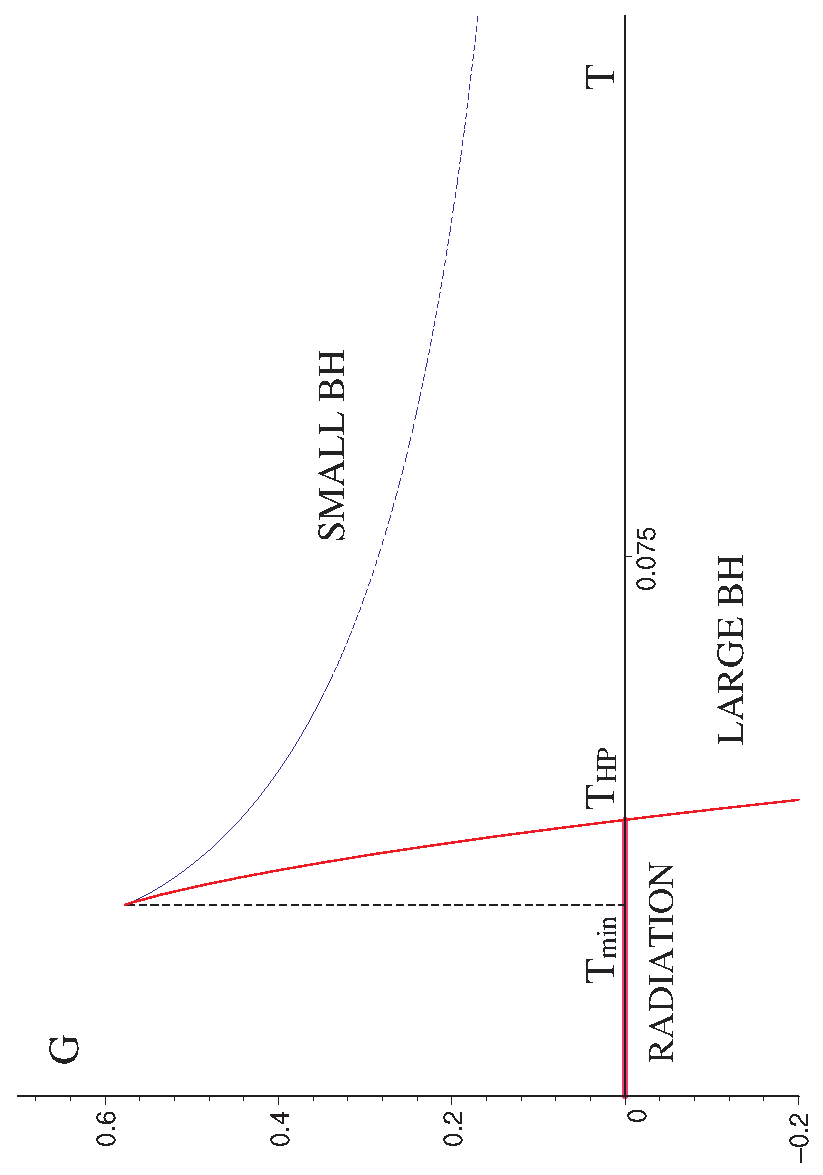
\includegraphics[width=0.4\textwidth,height=0.3\textheight]{Figures/HPG.eps}
}
\caption{{\bf Gibbs free energy: Schwarzchild-AdS black hole.}
When compared to the asymptotically flat Schwarzschild case (fig.~\ref{Fig:Gschflat}) for $P>0$ the Gibbs free energy acquires a new thermodynamically stable branch 
of large black holes. For $T>T_{\mbox{\tiny  HP}}$ this branch has negative Gibbs free energy and the corresponding black holes represent the 
globally thermodynamically preferred state. 
}
\label{Fig:Gschads}
\end{center}
\end{figure}

We observe a qualitatively different thermodynamic behaviour when compared to the asymptotically flat Schwarzschild case. Specifically $C_P$ is no longer always negative: it becomes positive for large (when compared to the AdS radius) black holes
\be
r_+>r_{\mbox{\tiny  min}}=\frac{l}{\sqrt{3}}\,,
\ee
while it is negative for $r_+<r_{\mbox{\tiny  min}}$ and ill defined at $r_+=r_{\mbox{\tiny  min}}$.




The behaviour of the Gibbs free energy $G$ is displayed in fig.~\ref{Fig:Gschads}.
We observe a minimum temperature $T_{\mbox{\tiny  \tiny min}}=2\sqrt{3}/(4\pi l)$, corresponding to $r_{\mbox{\tiny  min}}$, below which no black holes can exist. Above this temperature we have two branches of black holes. The upper one describes small (Schwarzschild-like) black holes with negative specific heat; these are thermodynamically unstable and  cannot be in a thermal equilibrium with a thermal bath of radiation. The large ($r_+>r_{\mbox{\tiny  \tiny min}}$) black holes at lower branch have positive specific heat and hence are locally thermodynamically stable. However, just above $T_{\mbox{\tiny  \tiny min}}$ the Gibbs free energy of such black holes is positive and the thermal AdS space with approximately zero Gibbs free energy represents a globally preferred thermodynamic state.\footnote{We refer to a thermal AdS space to be a (global) AdS space coupled to a bath of thermal radiation. Since the number of particle quanta representing the radiation is relatively small, the corresponding Gibbs free energy approximately equals zero.}     
This continues until temperature $T_{\mbox{\tiny  HP}}\approx 1/(\pi l)$ for which the black hole Gibbs free energy becomes negative, with the corresponding black hole radius given by 
\be
r_{\mbox{\tiny  HP}}=l\,.
\ee
Black holes with $r_+> r_{\mbox{\tiny  HP}}$ have negative Gibbs free energy and represent the globally preferred state. 
This means that at $T=T_{\mbox{\tiny  HP}}$ there is a first order {\em Hawking--Page} \cite{HawkingPage:1983} phase transition between thermal radiation and large black holes. This phase transition 
can be interpreted as a confinement/deconfinement phase transition in the dual quark
gluon plasma \cite{Witten:1998b}. 



Considering an extended phase space, the coexistence line of thermal radiation/large black hole phases, determined from $G=0$,
reads 
\be\label{HPcoexistence}
P|_{\mbox{\tiny  coexistence}}=\frac{3\pi}{8} T^2\,.
\ee
The corresponding $P-T$ phase diagram is displayed in fig.~\ref{Fig:HPtrans}.    
\begin{figure}
\begin{center}
\rotatebox{-90}{
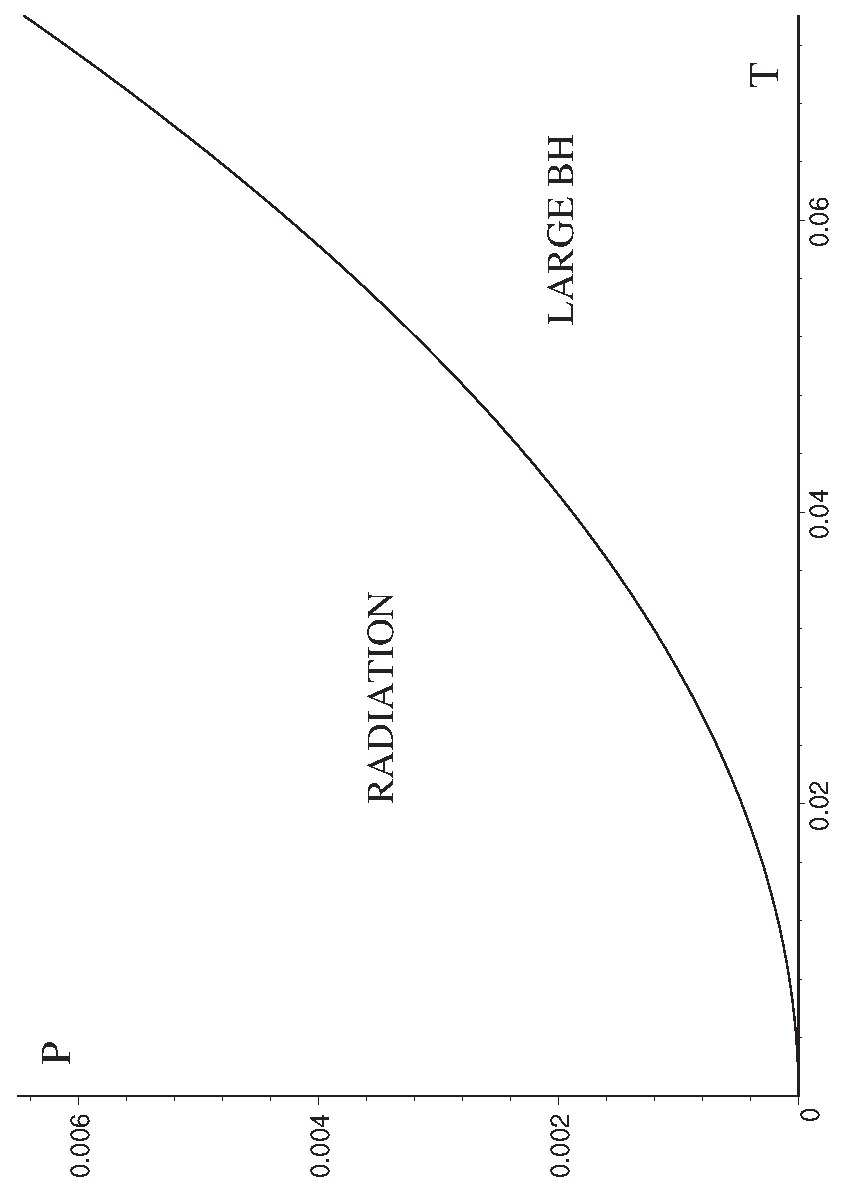
\includegraphics[width=0.4\textwidth,height=0.3\textheight]{Figures/HPtransition.eps}
}
\caption{{\bf Hawking--Page transition} is a first-order phase transition between thermal radiation in AdS and large stable Schwarzschild-AdS black hole. It occurs when $G$ of the Schwarzschild-AdS black hole approximately vanishes. Considering various pressures $P$ gives the radiation/large black hole coexistence line \eqref{HPcoexistence}  displayed in this figure. Similar to a ``solid/liquid'' phase transition, this line continues all the way to infinite pressure and temperature. 
}
\label{Fig:HPtrans}
\end{center}
\end{figure}


\begin{figure}
\begin{center}
\rotatebox{-90}{
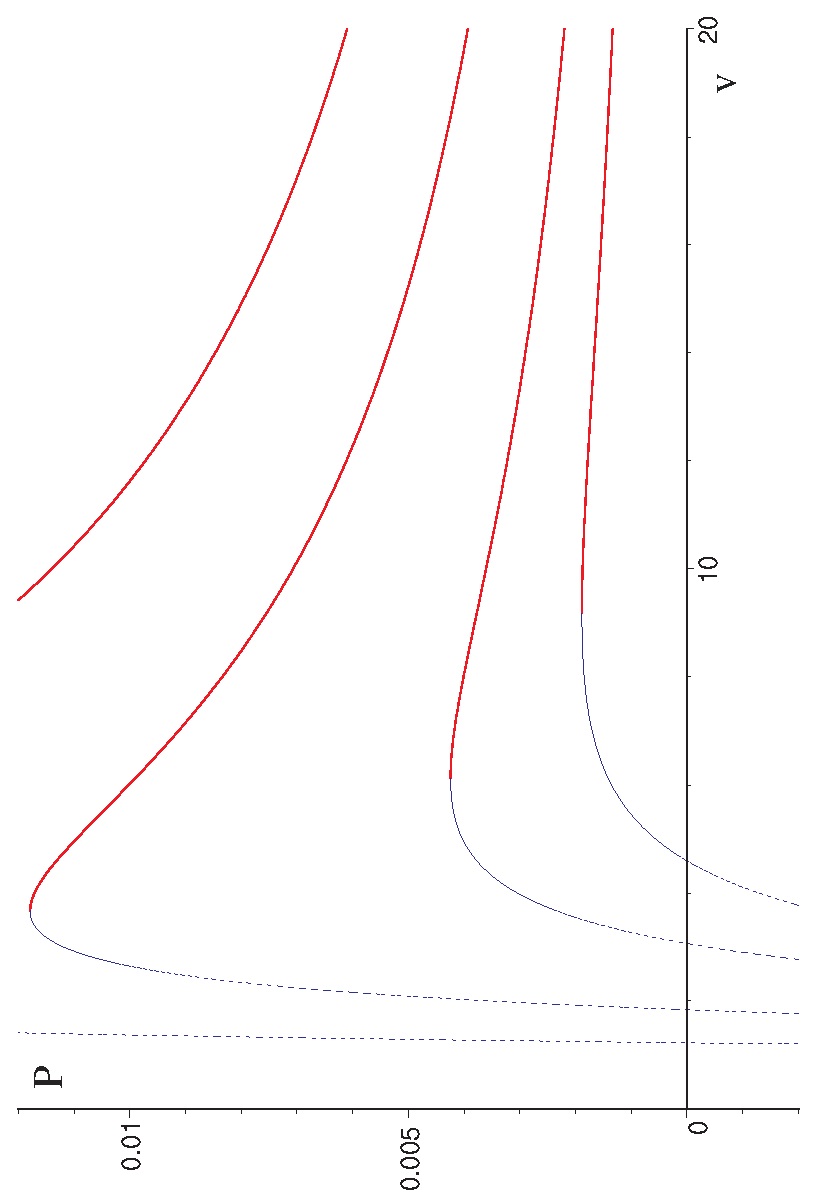
\includegraphics[width=0.4\textwidth,height=0.3\textheight]{Figures/HPstate.eps}
}
\caption{{\bf Equation of state: Schwarzschild-AdS black hole}. The equation of state \eqref{HPstate} is displayed for various temperatures. 
For a given temperature the maximum occurs at $v=2r_0$. The dashed blue curves correspond to small unstable black holes. The red curves depict the stable large black hole branch; we observe   `ideal gas' behaviour for large temperatures. 
}
\label{Fig:PVSchwAdS}
\end{center}
\end{figure}
By rewriting the temperature equation \eqref{SchaAdS} while using \eqref{PLambda}, we get a corresponding `fluid equation of state' 
for the Schwarzschild-AdS black hole, given by 
\be\label{HPstate}
P=\frac{T}{v}-\frac{1}{2\pi v^2}\,,\quad v=2\Bigl(\frac{3V}{4\pi}\Bigr)^{1/3}=2r_+\,.
\ee     
 The behaviour of this equation is displayed in the $P-V$ diagram in fig.~\ref{Fig:PVSchwAdS}. For each isotherm there is a maximum which occurs for $v=1/(\pi T)$. For a given temperature this precisely corresponds to $r_+=r_{\mbox{\tiny  \tiny min}}$; 
the dashed blue curves with positive slope (and possibly negative pressures) to the left of the maximum correspond to small black holes with negative $C_P$ which are thermodynamically unstable, whereas solid red curves correspond to large black holes with positive $C_P$ that are locally thermodynamically stable.



Let us compare the fluid equation of state of the Schwarzschild-AdS black hole \eqref{HPstate} with the famous {\em Van der Waals (VdW) equation}, e.g. \cite{Goldenfeld:1992},  which is a popular two parameter closed form modification of the ideal gas law that approximates the behaviour of real fluids. The VdW equation takes into account the nonzero size of fluid molecules 
(described by a constant $b>0)$ and the attraction between them (described by a constant $a>0$) and is often used to capture basic qualitative features of the liquid--gas phase transition. The equation reads (setting the Boltzmann constant $k_B=1$)
\be\label{VdW}
P=\frac{T}{v-b}-\frac{a}{v^2}\,,
\ee
where $v=V/N$ is the specific volume of the fluid, $P$ its pressure, $T$ its temperature, and the fluid parameters $a$ and $b$ are characteristics 
of a given fluid. The characteristic VdW $P-v$ diagram is displayed in fig.~\ref{fig:PVVdWstate}.
The equation admits a critical point, described by $\{T_c, v_c, P_c\}$, with universal critical ratio 
\be\label{universalVdWratio}
\rho_c=\frac{P_c v_c}{T_c}=\frac{3}{8}\,,
\ee
and the mean field theory critical exponents \eqref{MFT}.
\begin{figure}\label{fig:Fig1}
\begin{center}
\rotatebox{-90}{
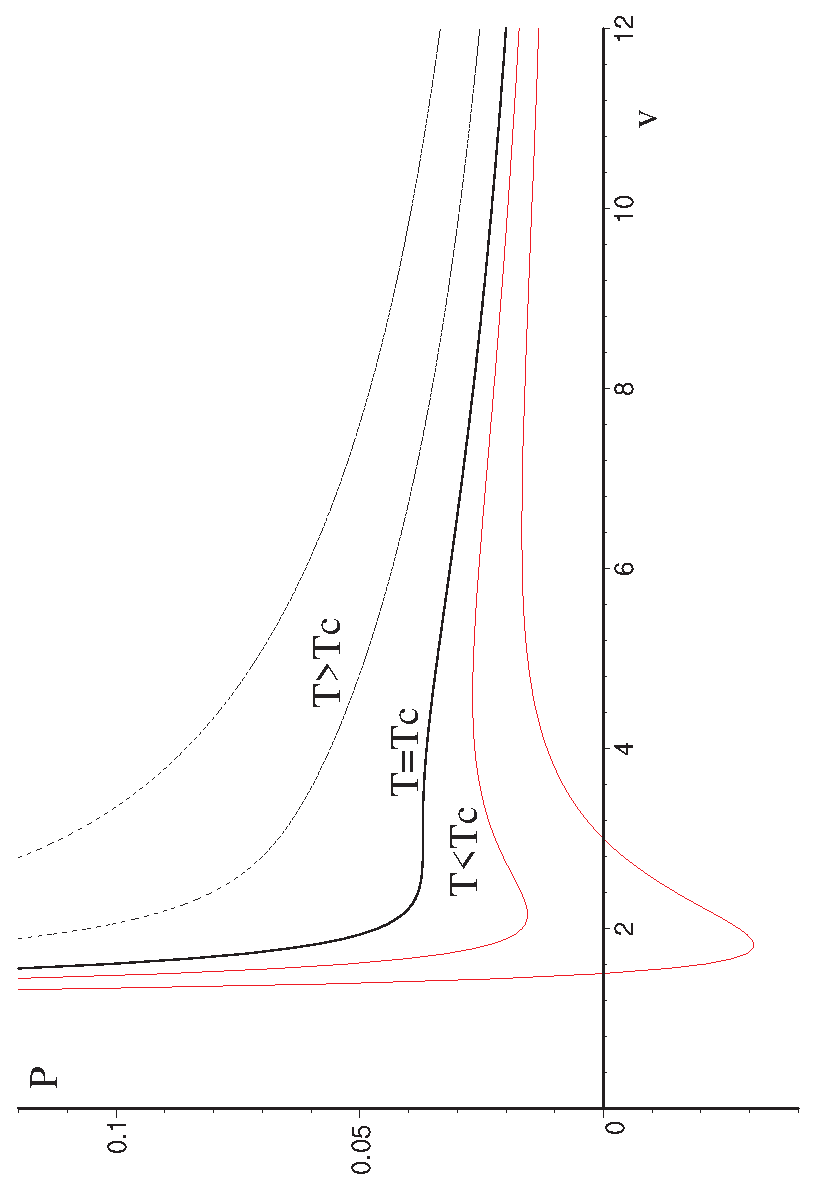
\includegraphics[width=0.39\textwidth,height=0.32\textheight]{Figures/PVVdW.eps}
}
\caption{{\bf $P-v$ diagram of Van der Waals fluid.} The temperature of isotherms decreases from top to bottom. The two upper dashed lines correspond to the ``ideal gas'' phase for $T>T_c$, the critical isotherm $T=T_c$ is denoted by the thick solid line, lower solid lines correspond to temperatures smaller than the critical temperature; for $T<T_c$ parts of the isotherms are actually unphysical, and must be replaced by a constant pressure line according to the Maxwell's equal area prescription \cite{KubiznakMann:2012}. Constants $a$ and $b$ were set equal to one.  
}  \label{fig:PVVdWstate}
\end{center}
\end{figure} 

We pause to consider topological Schwarzschild-AdS black holes.  Making use of the metric \eqref{ss} for arbitrary $k$, the 
formulae \eqref{SchaAdS} take the following more general form:
\ba
M &=& \frac{r_+ A_k}{8}\Bigl(k + \frac{r^2_+}{\ell^2}\Bigr)\,, \quad S=\frac{\pi A_k}{4} r^2_+\,, \nonumber\\
T &=& \frac{k \ell^2 + 3r^2_+}{4\pi\ell^3 r_+}\,,\quad V = \frac{\pi A_k}{3} r^3_+ \,,
\ea
where  $A_k$ is the area of the constant-curvature space divided by $\pi$; for a sphere, $A_{k=1} = 4$, 
for a torus, $A_{k=0} = A B$, where $A$ and $B$ and the sides of the torus, and there is no nice simple formula for $A_{k=-1}$.
In all cases the Smarr formula \eqref{Smarr} and first law \eqref{1st} hold.
It is then straightforward to show that the fluid corresponding to the  Schwarzschild-AdS black hole is characterized by
\be
a=\frac{k}{2\pi}\,,\quad b=0\,.
\ee
That is, its equation of state differs from the ideal gas law by the presence of a nontrivial parameter $a=k/(2\pi)$. This is directly related to the  topology of the horizon. For {\em planar} Schwarzschild-AdS black holes, $k=0$ and we recover the ideal gas law characterized by $a=0=b$, 
\be
Pv=T\,,
\ee
whereas for the $k=-1$ hyperbolic case we get a peculiar `repulsion' feature $a=-\frac{1}{2\pi}<0$, with $b=0$, the volume of molecules still vanishing.

We note one more interesting fact  for the planar ($k=0)$ AdS black holes.   In this case the following specific Smarr-like relation has been employed  e.g., \cite{Bertoldi:2010ca,Berglund:2011cp}:
\be\label{differentSmarr}
3 M=  2 TS\,,
\ee
[or $(d-1) M=(d-2) TS$ in  $d$-dimensions] without any reference to the $PV$ term. 
The value of our  Smarr relation \eqref{Smarr} is that it follows from the general geometric argument and 
applies to a wide class of (even possibly unknown) solutions that satisfy the assumptions of the theorem, whereas \eqref{differentSmarr} is a `phenomenological' observation valid for a particular sub-class of solutions. We also note that this relation is not related to the corresponding 
first law, $dM=TdS$, by a dimensional scaling argument.


 \subsection{Reissner–Nordstrom Solution}
 The charged AdS black hole metric is described by \eqref{ss} with
\be
f=1-\frac{2M}{r}+\frac{Q^2}{r^2}+\frac{r^2}{l^2}\,.
\ee
The thermodynamic quantities are 
\ba
T&=&\frac{1}{4\pi r_+^3 l^2}\Bigl(l^2(r_+^2-Q^2)+3r_+^4\Bigr)\,,\quad S=\pi r_+^2\,,\nonumber\\
V&=&\frac{4}{3}\pi r_+^3\,,\quad \Phi=\frac{Q}{r_+}\,,\quad 
G=\frac{l^2r_+^2-r_+^4+3Q^2l^2}{4l^2r_+}\,,\nonumber\\
C_P&=&2\pi r_+^2\frac{3r_+^4+l^2r_+^2-Q^2l^2}{3r_+^4-l^2r_+^2+3Q^2l^2}\,.
\ea
The specific heat is negative for 
\be
\frac{l \sqrt{1-\sqrt{1-36Q^2/l^2}}}{\sqrt{6}}<r_+<\frac{l \sqrt{1+\sqrt{1-36Q^2/l^2}}}{\sqrt{6}}\,,
\ee
and positive otherwise.


\begin{figure}
\begin{center}
\rotatebox{-90}{
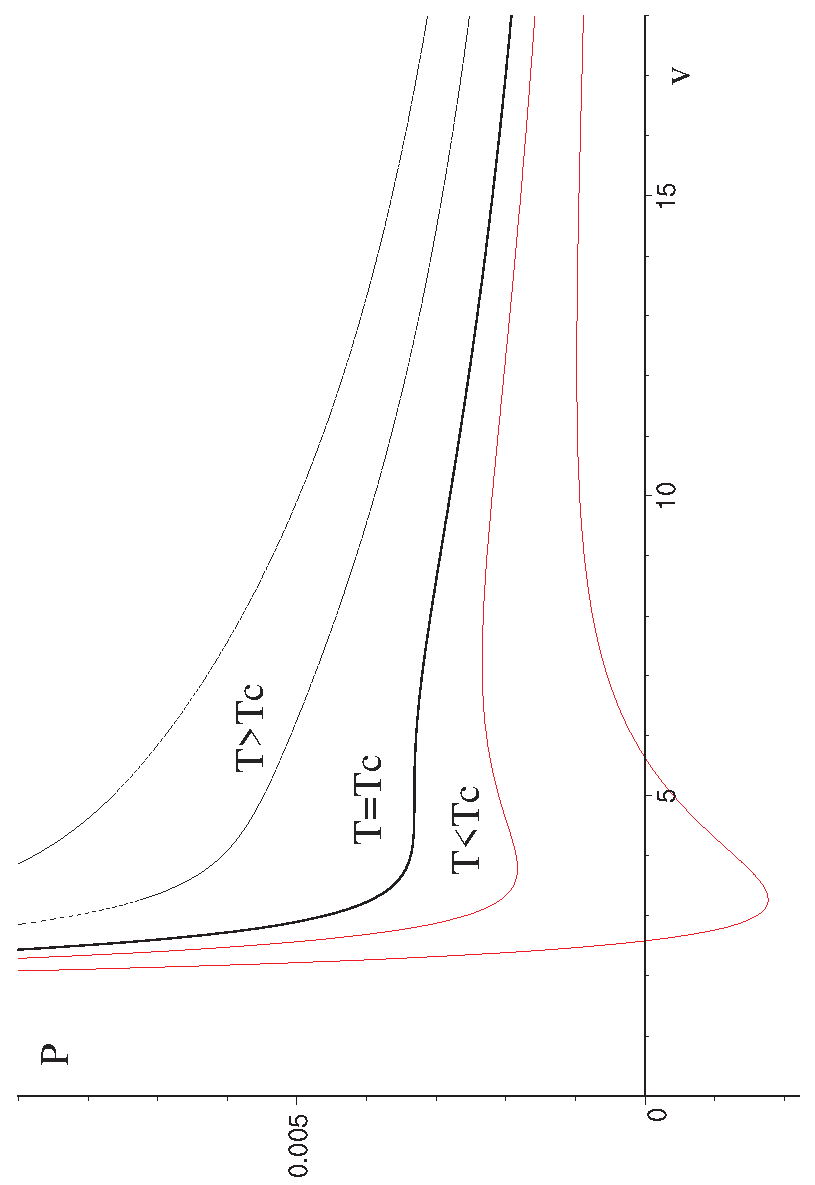
\includegraphics[width=0.39\textwidth,height=0.34\textheight]{Figures/rP.eps}
}
\caption{{\bf Equation of state: charged AdS black hole.}
The temperature of isotherms decreases from top to bottom. The two upper dashed lines correspond to the ``ideal gas'' one-phase behaviour for $T>T_c$, the critical isotherm $T=T_c$ is denoted by the thick solid line, lower solid lines correspond to temperatures smaller than the critical temperature.  We have set $Q=1$.  
$P-v$ diagram for the Kerr-AdS black hole with $J=1$ is qualitatively similar.
}\label{Fig:RNstate}
\end{center}
\end{figure} 
It was first noticed in \cite{ChamblinEtal:1999a,ChamblinEtal:1999b} that in a canonical (fixed charge) ensemble, charged AdS black holes allow for a first order {\em small-black-hole/large-black-hole} phase (SBH/LBH) transition which is in many ways reminiscent of the liquid/gas transition of a Van der Waals fluid.
This analogy becomes more complete in extended phase space \cite{KubiznakMann:2012}. 
Namely, the equation of state,
\be\label{RNstate}
P=\frac{T}{v}-\frac{1}{2\pi v^2}+\frac{2Q^2}{\pi v^4}\,,\quad v=2r_+\,,
\ee
mimics qualitatively the behaviour of the Van der Waals equation, shown in fig. \ref{fig:PVVdWstate}, with its black hole counterpart \eqref{RNstate} illustrated in fig. \ref{Fig:RNstate}.
Below $P_c$, the Gibbs free energy displays a characteristic swallowtail behaviour, depicted in fig.~\ref{Fig:Grnads}, indicating a first-order SBH/LBH phase transition. The corresponding coexistence line is displayed in fig.~\ref{Fig:RNPT}. 
It terminates at a critical critical point, characterized by 
\be
T_c=\frac{\sqrt{6}}{18\pi Q}\,,\quad v_c=2\sqrt{6} Q\,,\quad P_c=\frac{1}{96\pi Q^2}\,, 
\ee
where the phase transition becomes of the second order \cite{Banerjee:2010bx, MoLiu:2013}, and is characterized by the mean field theory critical exponents \eqref{MFT}. Remarkably the relation $\rho_c=P_c v_c/T_c=3/8$ is identical to  the Van der Waals case. The overall situation reminds one of the liquid/gas phase transition.  
A similar situation occurs for charged AdS black holes in higher dimensions \cite{GunasekaranEtal:2012}. 
\begin{figure}
\begin{center}
%\rotatebox{-90}{
\includegraphics[width=0.4\textwidth,height=0.3\textheight]{Figures/GrnAdS.eps}
%}
\caption{{\bf Gibbs free energy: charged AdS black hole.}
Characteristic swallowtail behaviour is observed for $P<P_c$, corresponding to a small/large black hole phase transition.
An unstable branch of the Gibbs free energy is displayed in dashed blue line. We have set $Q=1$.
The behaviour of $G$ for Kerr-AdS black hole with $J=1$ is qualitatively similar.
}
\label{Fig:Grnads}
\end{center}
\end{figure}
\begin{figure}
\begin{center}
\rotatebox{-90}{
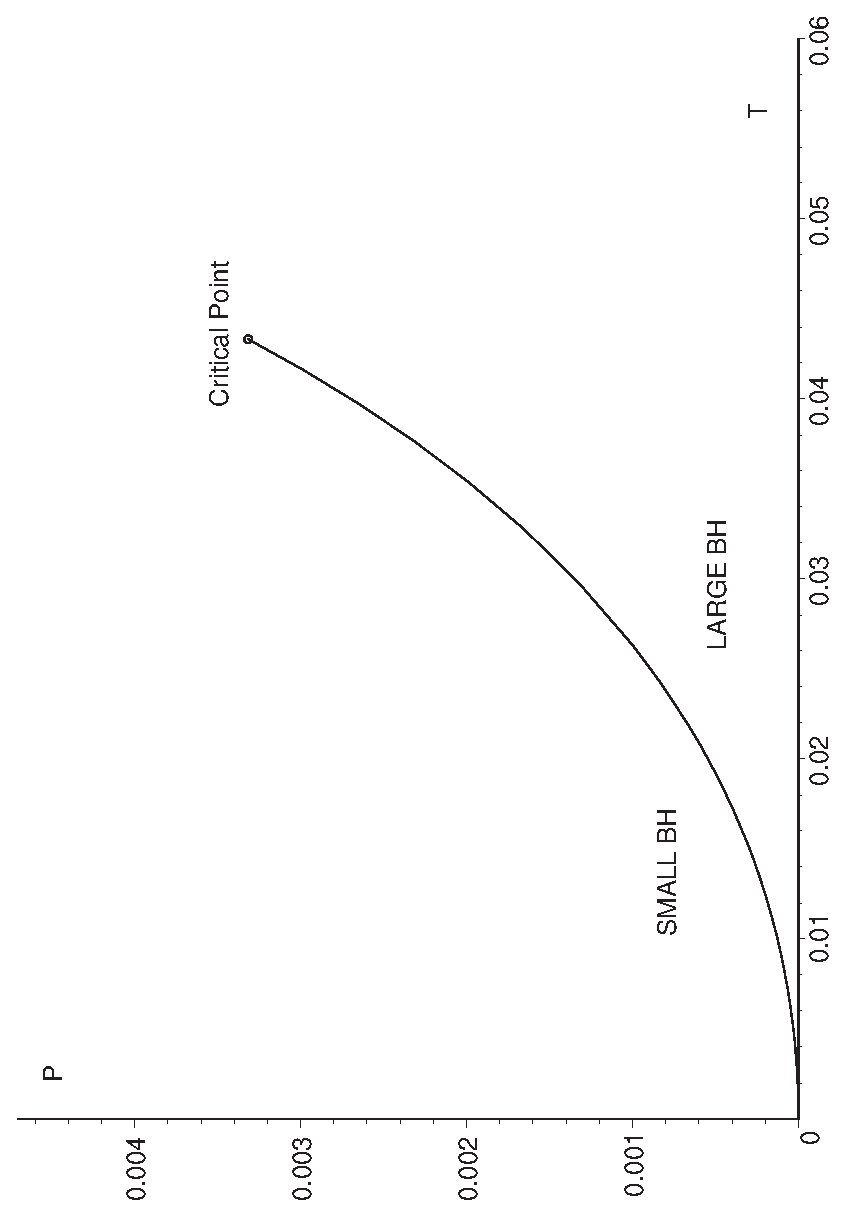
\includegraphics[width=0.39\textwidth,height=0.34\textheight]{Figures/PT2.eps}
}
\caption{{\bf Phase diagram: charged AdS black hole.} The coexistence line of the SBH/LBH phase transition of the charged AdS black hole system in $(P, T)$-plane is displayed. The critical point is highlighted by a small circle at the end of the coexistence line. The
phase diagram for a Kerr-AdS black hole with $J=1$ is qualitatively similar.
} \label{Fig:RNPT} 
\end{center}
\end{figure} 

We remark that the Hawking--Page phase transition as well as the SBH/LBH phase transition ala Van der Waals can be also observed for asymptotically flat or de Sitter charged black holes provided these are placed in a finite cavity \cite{Carlip:2003ne}.  



We close this subsection by noting that strongly charged small AdS black holes are subject to superradiant instabilities. For a charged scalar field coupled to Einstein--Maxwell theory a similar situation occurs:  
at small temperatures  charged scalar hair forms and the resulting `hairy black holes' are thermodynamically preferred  \cite{Gubser:2008px, Hartnoll:2008vx, Hartnoll:2008kx, Maeda:2010hf, Basu:2010uz, Dias:2011tj, Horowitz:2010gk, Hartmann:2013nla}. This means that in the presence of a charged scalar field, the left-most branch of small black holes in the Gibbs free diagram \ref{Fig:Grnads}, although locally thermodynamically stable, does not globally minimize the Gibbs free energy. Rather, there is another branch of hairy black holes with 
lower Gibbs free energy. The hair/no-hair black hole phase transition is of the second order and underlies the theory of holographic superconductors.   

  

 \subsection{Kerr Solution}
 
 
The thermodynamics of four-dimensional rotating AdS black holes is qualitatively similar to the charged AdS case.\footnote{In fact a qualitatively similar behaviour occurs for charged rotating AdS black holes, see \cite{CaldarelliEtal:2000}.} 
The metric is  
\begin{eqnarray}
ds^2&=&-\frac{\Delta}{\rho^2}(dt-\frac{a}{\Xi}\sin^2\!\theta d\varphi)^2+
\frac{\rho^2}{\Delta}dr^2+\frac{\rho^2}{\Sigma}d\theta^2 \nonumber \\
&+&
\frac{\Sigma \sin^2\!\theta}{\rho^2}[adt-\frac{(r^2+a^2)}{\Xi}d\varphi]^2\,,
\end{eqnarray}
where
\begin{eqnarray}
\Delta&=&(r^2+a^2)(1+\frac{r^2}{l^2})-2mr\,,\quad
\Sigma=1-\frac{a^2}{l^2}\cos^2\theta \,,\nonumber \\
\Xi&=&1-\frac{a^2}{l^2}\,, \quad
\rho^2=r^2+a^2\cos^2\theta \,. \nonumber
\end{eqnarray}
The thermodynamic quantities read 
\begin{eqnarray}
M&=&\frac{m}{\Xi^2}\,, \quad J=\frac{ma}{\Xi^2} \,, \quad  \Omega=\frac{a}{l^2}\frac{r_+^2+l^2}{r_+^2+a^2}\,, \nonumber\label{OHJ}\\
T&=&\frac{1}{2\pi r_+}\Bigr[\frac{(a^2+3r_+^2)(r_+^2/l^2+1)}{2(a^2+r_+^2)}-1\Bigr]\,, \nonumber\label{BHT} \\
S &=&\pi \frac{(a^2+r_+^2)}{\Xi}=\frac{A}{4} \,,\quad V=\frac{r_+A}{3}\Bigl(1+\frac{1+r_+^2/l^2}{2r_+^2}\frac{a^2}{\Xi}\Bigr)\,, \nonumber\label{BHS}\\
G &=& \frac{(r^2_+ + 3a^2) l^4 -(r^2_+ - a^2)^2 l^2 + (a^2 + 3 r^2_+)a^2 r^2_+}{l^4 \Xi^2 r_+}\,, \nonumber \\
\end{eqnarray}
and satisfy the Smarr relation \eqref{Smarr}; 
rather lengthy formula for $C_P$ can be found in \cite{MonteiroEtal:2009}.
%\ba
%C_P=-\frac{2\pi l^4(a^2+r_+^2)^2[(r_+^2-l^2)a^2+r_+^2(l^2+3r_+^2)]}
%{(a^2-l^2)[(3a^4+6r_+^2a^2-r_+^4)l^4+(a^6+13r_+^2a^4+23r_+^4a^2+3r_+^6)l^2
%+a^2r_+^2(a^2+3r_+^2)^2]}\,.
%\ea

The Gibbs free energy, equation of state, and the $P-T$ phase diagram are qualitatively similar to figs.~\ref{Fig:Grnads}, \ref{Fig:RNstate} and 
\ref{Fig:RNPT}---with fixed $J$ replacing fixed $Q$.  For any fixed $J$, there is a critical point, characterized by $(P_c, V_c, T_c)$, that can be determined numerically. For $P<P_c$, the Gibbs free energy displays  swallowtail behaviour and there is a corresponding SBH/LBH first order phase transition with a phase diagram similar to fig.~\ref{Fig:RNPT}. It will be shown in the next section that in the limit of slow rotation,  $a\ll l$, the equation of state can be approximated by 
\ba
P&=&\frac{T}{v}-\frac{1}{2\pi v^2}+\frac{48J^2}{\pi v^6}-\frac{384 J^4(7+8\pi Tv)}{(1+\pi Tv)^2\pi v^{10}}\nonumber\\
&&+\frac{36864(13\pi Tv\!+\!11)J^6}{\pi v^{14}(1+\pi Tv)^3}\!+\!O\bigl[(a/l)^8\bigr]\,,\nonumber \\
v&=&2\Bigl(\frac{3V}{4\pi}\Bigr)^{\!1/3}\,.
\ea
The first three terms were first obtained in \cite{GunasekaranEtal:2012}. Using this equation of state, one can approximately find 
the critical point and study its characteristics. In particular, one finds that the critical exponents 
remain as predicted by the mean field theory, given by \eqref{MFT}. 

We pause to remark that, similar to the charged AdS case, the rotating AdS black holes close to extremity are unstable with respect to   superradiant instabilities;  the resultant objects (hairy black hole, soliton, or boson star) are expected to globally minimize the Gibbs free energy \cite{Hawking:1999dp, Sonner:2009fk, Dias:2010ma, Cardoso:2013pza}.




 \subsection{general solution }
 
 
 \subsection{Higher-dimensional Kerr-AdS black hole spacetimes}
General Kerr-AdS black hole spacetimes \cite{GibbonsEtal:2004, GibbonsEtal:2005}  are $d$-dimensional metrics that solve the Einstein equations with  cosmological constant
\be
R_{ab} =\frac{2\Lambda}{(d-2)}  g_{ab}
\ee
and generalize the $d$-dimensional asymptotically-flat rotating black hole spacetimes of Myers and Perry \cite{MyersPerry:1986}.   
In   Boyer--Lindquist  coordinates the metric takes the form
\ba \label{metric}
ds^2&=&-W\Bigl(1+\frac{r^2}{l^2}\Bigr)d\tau ^2+\frac{2m}{U} \Bigl(W d\tau -\sum_{i=1}^{N} \frac{a_i \mu_i ^2 d\varphi _i}{\Xi _i}\Bigr)^2\nonumber\\
&+&\sum_{i=1}^{N} \frac{r^2+a_i^2}{\Xi _i} \mu_i ^2 d\varphi _i^2+\frac{U dr^2}{F-2m}+\sum_{i=1}^{N+\varepsilon}\frac{r^2+a_i ^2}{\Xi _i} d\mu _i ^2 \nonumber\\
&-&\frac{l^{-2}}{W (1+r^2/l^{2})}\Bigl(\sum_{i=1}^{N+\varepsilon}\frac{r^2+a_i ^2}{\Xi _i} \mu_i d\mu_i\Bigr)^2\,,
\ea
where 
\ba\label{metrcifunctions}
W&=&\sum_{i=1}^{N+\varepsilon}\frac{\mu _i^2}{\Xi _i}\,,\quad U=r^\varepsilon \sum_{i=1}^{N+\varepsilon} \frac{\mu _i^2}{r^2+a_i^2} \prod _j ^N (r^2+a_j^2)\,,\nonumber\\
F&=&r^ {\varepsilon -2} \Bigl(1+\frac{r^2}{l^2}\Bigr) \prod_{i=1}^N (r^2+a_i^2)\,,\quad \Xi_i=1-\frac{a_i^2}{l^2}\,.\quad
\ea
To treat even ($\varepsilon=1)$  odd ($\varepsilon=0)$ spacetime dimensionality $d$ simultaneously, we have parametrized
\be
d=2N + 1 + \varepsilon\,,
\ee 
and in even dimensions set for convenience $a_{N+1}=0$.
The  coordinates $\mu_i$ are not independent, but obey the constraint
\begin{equation}\label{constraint}
\sum_{i=1}^{N+\varepsilon}\mu_i^2=1\,.
\end{equation}
In general the spacetime admits $N$ independent angular momenta $J_i$, described by
$N$ rotation parameters $a_i$, and generalizes the previously known singly-spinning case \cite{HawkingEtal:1999}.
In $d=4$ it reduces to the four-dimensional Kerr-AdS metric studied in the previous section.  
With this metric it shares a remarkable property---it possesses a hidden symmetry associated with the Killing--Yano tensor \cite{KubiznakFrolov:2007} that is responsible for integrability of geodesic motion and various test field equations in these spacetimes, see, e.g., review \cite{FrolovKubiznak:2008}.

 

The thermodynamic quantities associated with Kerr-AdS black holes were first calculated in \cite{Gibbons:2004ai}.
The mass $M$, the angular momenta $J_i$, and the angular velocities of the horizon $\Omega_i$ read
\ba \label{TD}
M&=&\frac{m \omega _{d-2}}{4\pi (\prod_j \Xi_j)}\bigl(\sum_{i=1}^{N}{\frac{1}{\Xi_i}-\frac{1-\varepsilon }{2}}\bigr)\,,\nonumber\\
J_i&=&\frac{a_i m \omega _{d-2}}{4\pi \Xi_i (\prod_j \Xi_j)}\,,\quad \Omega_i=\frac{a_i (1+\frac{r_+^2}{l^2})}{r_+^2+a_i^2}\,,
\ea
while the temperature $T$, the horizon area $A$, and the entropy $S$ are given by
\ba\label{TS}
T&=&\frac{1}{2\pi }\Bigr[r_+\Bigl(\frac{r_+^2}{l^2}+1\Bigr)
\sum_{i=1}^{N} \frac{1}{a_i^2+r_+^2}-\frac{1}{r_+}
\Bigl(\frac{1}{2}-\frac{r_+^2}{2l^2}\Bigr)^{\!\varepsilon}\,\Bigr]\,,\nonumber\\
A&=&\frac{\omega _{d-2}}{r_+^{1-\varepsilon}}\prod_{i=1}^N 
\frac{a_i^2+r_+^2}{\Xi_i}\,,\quad S=\frac{A}{4}\,. 
\ea
The horizon radius $r_+$ is determined as the largest root of $F-2m=0$ and $\omega_{d}$ is given by \eqref{omega}.


The thermodynamic volume reads \cite{CveticEtal:2010, Dolan:2013}
\begin{eqnarray} \label{VBHKerr}
V& =& \frac{r_+ A }{d-1}\left[1+\frac{1+{r^2_+}/{l^2}}{(d-2)r_+^2}\sum_i \frac{a_i^2}{\Xi_i}\right]  \nonumber\\ \label{VBHKerr2}
&=&	{\frac{r_+ A }{d-1}+{8\pi\over (d-1)(d-2)}\sum_i a_iJ_i }\,, 
\end{eqnarray}
and indeed is required to ensure that the Smarr formula \eqref{Smarr} holds.
It is known to obey the {\em reverse isoperimetric inequality} \eqref{ISO} provided that in \eqref{ratio} we identify ${\cal A}=A$ and ${\cal V}=V$
as given by \eqref{TS} and \eqref{VBHKerr}.
In fact the inequality is saturated for non-rotating black holes, whereas it becomes most extreme $({\cal R}\to \infty)$
in the ultraspinning limit, see discussion around Eq. \eqref{ratioInfinity}.


Note that the `naive' {\em geometric volume} \cite{Parikh:2006, BallikLake:2010, CveticEtal:2010,BallikLake:2013} (given by the spatial integral of $\sqrt{-g}$ integrated up to the horizon radius) 
\be
V'=\frac{r_+ A}{d-1}\,
\ee
and the thermodynamic volume $V$ in \eqref{VBHKerr} differ by an $\sum_i a_iJ_i$ term and behave differently in the limits of slow and fast rotation. 
Whereas the thermodynamic volume \eqref{VBHKerr} is dominated by its first geometric term for slow rotations 
\be\label{Vslow}
V_{\mbox{\tiny  slow}}\approx V'_{\mbox{\tiny  slow}}\approx\frac{\omega_{d-2}r_+^{d-1}}{d-1}\,,
\ee
in the ultraspinning regime the second (angular momentum) term dominates.
To see this let us, for simplicity, consider for a moment 
a singly spinning Myers--Perry black hole ($a_1=a$, other $a_i=0$, and $l\to \infty$). 
In this case the formula \eqref{VBHKerr} reduces to  the following expression 
\be\label{VKerr}
V=V'+\frac{4\pi}{d-1}\frac{J^2}{M}
\ee
which is also valid for the $d=4$ Kerr-AdS case.
In $d\geq 6$ there is no limit on how large the rotation parameter $a$ can be \cite{EmparanMyers:2003} and one can, in principle, take the {\em ultraspinning limit} $a\to \infty$. For fixed $M$ this implies $r_+\to 0$, and the second term in the previous formula dominates.
Hence, for the ultraspinning black holes, the thermodynamic volume differs significantly from the geometric one, being approximately given by
\be\label{VeqV'}
V\approx \frac{4\pi}{d-1}\frac{J^2}{M}\approx \frac{\omega_{d-2} a^4 r_+^{d-5}}{(d-1)(d-2)}\,,
\ee
which is to be compared with formula \eqref{Vslow}. The conclusions for multiply-spinning and/or AdS black holes are   analogous.

The Gibbs free energy is given by \eqref{G} and is related to the Euclidean action $I$ \cite{Gibbons:2004ai},  
\be\label{action}
I=\frac{\omega_{d-2}}{8\pi T\bigl(\prod_j \Xi_j\bigr)}\Bigl(m-\frac{r_+^\varepsilon}{l^2}\prod_{i=1}^N(r_+^2+a_i^2)\Bigr)\,,
\ee
by 
\be\label{GibbsKerrAdS}
G=M-TS=TI+\sum_{i}\Omega_i J_i\,,
\ee
see also Sec.~\ref{sec:Instab} where $I$ is used to estimate the onset of ultraspinning instabilities.  
In what follows we shall discuss in detail some special cases of these general metrics and the associated interesting thermodynamic features.


\section {Géométrie thermodynamique et transition de phase}

 Une autre approche pour étudier le comportement thermodynamique du système est la géométrie thermodynamique. Cette méthode nécessite une métrique appropriée en utilisant des quantités thermodynamiques. Pour construire une métrique appropriée, on peut utiliser un potentiel thermodynamique avec
ensemble spécifique de paramètres étendus. Puis en calculant le scalaire de Ricci de la métrique introduite
et en déterminant les points de divergence, on peut étudier les deux types de transition de phase. Il
a été démontré que le résultat obtenu est similaire au résultat de la capacité calorifique. Ça veut dire
les points de divergence du scalaire de Ricci et la divergence / point zéro de la capacité thermique coïncident.\\
Comme mentionné en introduction, il existe plusieurs méthodes pour construire un espace-temps géométrique telles que
Métrique Weinhold, Ruppeiner, Quevedo et HPEM. Nous passons d'abord en revue les quatre mesures mentionnées
et étudiez la transition de phase du trou noir chargé en accélération AdS chargé dans une phase non étendue
espace et espace de phase étendu. Ensuite, nous comparerons les résultats avec la capacité thermique et
trouvera la métrique appropriée pour étudier la transition de phase d'un trou noir chargé en accélération AdS.\\
Comme mentionné, nous considérons la charge électrique comme un paramètre fixe dans la transition de phase
de la capacité thermique dans un ensemble canonique. Mais la construction d'une métrique thermodynamique peut constituer une variable considérable. Pour trou noir accéléré chargé en AdS dans un espace de phase non étendu,
nous supposons que la pression est une quantité thermodynamique fixe et considérons la masse totale comme
potentiel thermodynamique et l'entropie et la charge électrique comme paramètres étendus. À présent
nous voulons étudier la transition de phase du trou noir accéléré chargé en AdS par ce qui précède
métriques thermodynamiques mentionnées.

\subsection{Métrique de Weinhold et Ruppeiner}
La première formulation géométrique a été introduite par Weinhold\cite{52}. Il a défini la métrique thermodynamique
 comme la dérivée seconde de la masse (énergie interne) par rapport à l'entropie et
d'autres paramètres étendus. La métrique de Weinhold est donnée par,
\begin{equation}
g_{ij}^{w}=\dfrac{\partial^{2}M(x^{k})}{\partial x^{i} \partial x^{j} };  x^{i}=(S,N^{a}) 
\end{equation}

où S est l'entropie et $N^{a}$ détermine toutes les autres variables étendues du système.\\
Cette métrique de Weinhold est conforme à la métrique de Ruppeiner 
avec  la température comme facteur conforme
\begin{equation}
g_{ij}^{w}= T g_{ij}^{R}
\end{equation}

la métrique de Ruppeiner \cite{53} est définie comme la dérivée seconde de l’entropie par rapport à l’énergie
interne et d’autres variables extensives. La metrique de Ruppeiner est défini par,
\begin{equation}
\label{xss}
g_{ij}^{R}=-\dfrac{\partial^{2}S(x^{k})}{\partial x^{i} \partial x^{j} }=\dfrac{1}{T}\dfrac{\partial^{2}M(x^{k})}{\partial x^{i} \partial x^{j} };  x^{i}=(U,N^{a}) 
\end{equation}

où U est l'entropie et $N^{a}$ détermine les variables extensives du système.\\
Dans l'espace des états on considère $x^{\mu} = (S, Q)$ comme variables extensives. Un calcul simple de courbure de la métrique\ref{xss} donne
\begin{equation}
R=-\dfrac{1}{\sqrt{g}}\left[\dfrac{\partial}{\partial S}\left( \dfrac{g_{SQ}}{g_{SS}\sqrt{g}}\dfrac{\partial g_{SS}}{\partial Q}-\dfrac{1}{\sqrt{g}}\dfrac{\partial g_{QQ}}{\partial S}\right)  +\dfrac{\partial}{\partial Q}\left( \dfrac{2}{\sqrt{g}}\dfrac{\partial g_{SQ}}{\partial S}-\dfrac{1}{\sqrt{g}}\dfrac{\partial g_{QQ}}{\partial S}-\dfrac{1}{\sqrt{g}}\dfrac{\partial g_{SS}}{\partial Q}-\dfrac{g_{SQ}}{g_{SS}\sqrt{g}}\dfrac{\partial g_{SS}}{\partial S}\right)\right] 
\end{equation}
Danc n peut exprimer le scalaire de Ricci de la  métrique de Ruppeiner  comme
\begin{equation}
R^{R}=\dfrac{8PS(8PS^{2}+\pi Q^{2})(S(8PS-3)+3\pi Q^{2})}{(S(8PS-1)+\pi Q^{2})^{2}(\pi Q^{2}-S(8PS+1))}
\end{equation}
nous avons tracé le scalaire  Ricci  de Ruppeineren ce qui concerne l'entropie dans les figures suivants\\

\begin{figure}[H]
%\includegraphics[scale=0.8]{images/metriqueR.png}
\caption{La courbure scalaire de la géométrie de Ruppeiner pour une transition de phase
	de première ordre $P < P_{c}$ (à gauche) et de deuxième ordre où $P = P_{c}$ (à droite) . On fixe Q = 1.}
\end{figure} 

Nous pouvons remarquer que le point de divergence n’est pas identique à celui de la
capacité thermique $(S_{min}, S_{max})$ pour $P < P_{c}$ et Sc pour$ P = P_{c}$. Par conséquent,
c'est à dire 
que le point de divergence n'est pas identique à la divergence / point zéro de la capacité calorifique, c'est pourquoi
Métrique n'est pas en mesure de décrire la transition de phase de cette solution de trou noir.
\subsection{Métrique de Quevedo}
Comme nous le savons, la métrique de Ruppeiner et la métrique de Weinhold ne sont pas invariantes sous Legendre.
transformation. Pour cette raison, Quevedo a introduit une métrique invariante de Legendre,
dans l'espace de l'état d'équilibre \cite{54}. Le Quevedo a deux types de métriques correspondantes
qui sont donnés par \cite{55},

\begin{equation}
dS_{Q}^{2}=g{ij}^{Q}dx^{i}dx^{j},
\end{equation}

Or $g_{ij}^{Q}$ est donnée par 
\begin{equation}
g{ij}^{Q}=\left( S\dfrac{\partial M}{\partial S}+Q\dfrac{\partial M}{\partial Q}\right)
\begin{pmatrix}
 -\dfrac{\partial^{2}M}{\partial S^{2}}  & 0\\
  0                                     & \dfrac{\partial^{2}M}{\partial Q^{2}}                  
\end{pmatrix}
\end{equation}

le scalaire de Ricci de cette métrique est

\begin{equation}
R_{ij}^{Q}=\dfrac{32\pi^{2} S^{2}\left(9\pi^{2}Q^{4}(28PS-1)+3\pi Q^{2}S(4PS(16PS-5)+3)+8PS^{3}(4PS(1-40PS)+1) \right) }{\left(-8PS^{2}-3\pi Q^{2}+S \right)^{2}\left(8PS^{2}+3\pi Q^{2}+S \right)^{3}  }
\end{equation}

nous avons tracé le scalaire  Ricci  de Quevedoen ce qui concerne l'entropie dans les figures suivants \\

\begin{figure}[H]
%	\includegraphics[scale=0.8]{images/metriqueQ.png}
	\caption{La courbure scalaire de la géométrie de Quevedo pour une transition de phase
		de première ordre $P < P_{c}$ (à gauche) et de deuxième ordre où $P = P_{c}$ (à droite) . On fixe Q = 1.}
\end{figure}

Il est clair que cette métrique présente des points de divergence qui coïncident avec
ceux de la capacité thermique. On peut dire que cette géométrie est capable de décrire la
transition de phase 1er/2ème ordre pour les trous noirs de RN-AdS.

\subsection{Métrique de Hendi, Panahiyan et Eslam HPEM}
En 2015 Hendi et ses collaborateurs ont introduit une nouvelle métrique \cite{56} qui contenait les deux types de transition de phase. C’est un métrique qui rectifie les lacunes de la
géométrie de Ruppeiner et Quevedo. La géométrie de HPEM est donnée par
\begin{equation}
g_{ij}^{HPEM}=\left( \dfrac{S M_{s}}{M_{QQ}^{3}}\right)
\begin{pmatrix}
-M_{SS}  & 0\\
0        & M_{QQ}
\end{pmatrix}
\end{equation}

Calculant le sclaire de HPEM Ricci,son dénominateur est 
\begin{equation}
demn(R_{HPEM})=S^{3}M_{S}^{3}M_{SS}^{2}
\end{equation}

On trace le scalir Ricci de HPEM  en fonction de l'entropie\\

\begin{figure}[H]
%	\includegraphics[scale=0.8]{images/matriqueH.png}
	\caption{La courbure scalaire de la géométrie de HPEM pour une transition de phase
		de première ordre $P < P_{c}$ (à gauche) et de deuxième ordre où $P = P_{c}$ (à droite) . On fixe Q = 1.}
\end{figure}

On peut voir que les points de divergence coïncident exactement avec les points de
divergence de la capacité calorifique ainsi que son point zéro. Alors on peut dire que cette
métrique peut décrire la transition de phase et déterminer le trou noir extrémal donné
par $C_{p} = 0$ ou T = 0.\\
\\
En étudiant la géométrie thermodynamique dans l'espace de phase, on remarque que
Ruppeiner n'est pas un candidat approprié pour étudier la transition de phase pour le
trou noir RN-AdS. Par contre les métriques HPEM et Quevedo sont capables de décrire
correctement la transition de phase thermodynamique.

 
 
